% !TeX spellcheck = it_IT
% !TEX TS-program = pdflatex
% !TEX root = ../main.tex


% ********************************************************************
\section{Implementazione e prototipo}
\label{sec:prototipo}
% ********************************************************************


\subsection{Login e autenticazione}
Il sistema di autenticazione della piattaforma è stato progettato seguendo un approccio \textit{wallet-based}, coerente con il paradigma Web3 e volto a eliminare l’utilizzo di credenziali tradizionali quali \textit{username} e \textit{password}. L’identità dell’utente è infatti associata in modo univoco al possesso di un \textit{wallet} blockchain. \\
Il processo di \textit{login} ha inizio con la connessione del \textit{wallet} dell’utente, dal quale viene ricavato l’indirizzo pubblico. A partire da tale indirizzo, il \textit{backend} genera un \textit{nonce}, ovvero un valore casuale e univoco, il quale viene associato all’indirizzo del \textit{wallet} e successivamente restituito al \textit{front-end}. \\
Il \textit{front-end} costruisce quindi un messaggio conforme allo standard \gls{siwe}, includendo il \textit{nonce} ricevuto, e richiede all’utente di firmarlo tramite il proprio wallet. La firma crittografica prodotta dimostra il possesso della chiave privata associata all’indirizzo e viene inviata al backend insieme al messaggio firmato. Il \textit{back-end} verifica la validità della firma ricostruendo il messaggio e accertando che: 
\begin{enumerate}
	\item l’indirizzo estratto crittograficamente dalla firma coincida con quello dichiarato;
	\item il \textit{nonce} contenuto nel messaggio corrisponda a quello precedentemente generato e memorizzato.
\end{enumerate}
Solo nel caso in cui entrambi i controlli diano esito positivo, l’autenticazione viene considerata valida e la sessione dell’utente viene inizializzata.\\
In fase di primo accesso, l’utente viene registrato automaticamente nel sistema, mentre per accessi successivi vengono aggiornate le informazioni di sessione. Al termine del processo, il nonce viene rigenerato, invalidando quello precedente e garantendo la sicurezza delle autenticazioni future.


\subsection{Dashboard donatore}
La \textit{dashboard} del donatore è l'interfaccia attraverso la quale gli utenti possono interagire direttamente con la piattaforma a seguito della procedura di autenticazione. Essa è progettata per fornire una visione sintetica e intuitiva delle iniziative di \gls{cf} attive, permettendo all'utente di monitorarne lo stato di avanzamento attraverso indicatori chiave quali il \textit{budget} raccolto, il numero di donatori coinvolti e la data di scadenza. \\
Una volta selezionata l’iniziativa di interesse, l’utente ha la possibilità di procedere con l’operazione di donazione. In particolare, il sistema adotta il meccanismo di raccolta \textit{keep-it-all}, in base al quale l’Ente beneficiario conserva i fondi raccolti anche qualora l’obiettivo economico prefissato non venga raggiunto entro i termini prestabiliti.
Tale scelta progettuale risulta coerente con la categoria di Enti autorizzati alla creazione delle iniziative sulla piattaforma, individuati esclusivamente negli Enti del Terzo Settore, per i quali anche contributi parziali possono risultare funzionali al perseguimento delle finalità sociali.


\begin{figure}[!h]
	\centering
	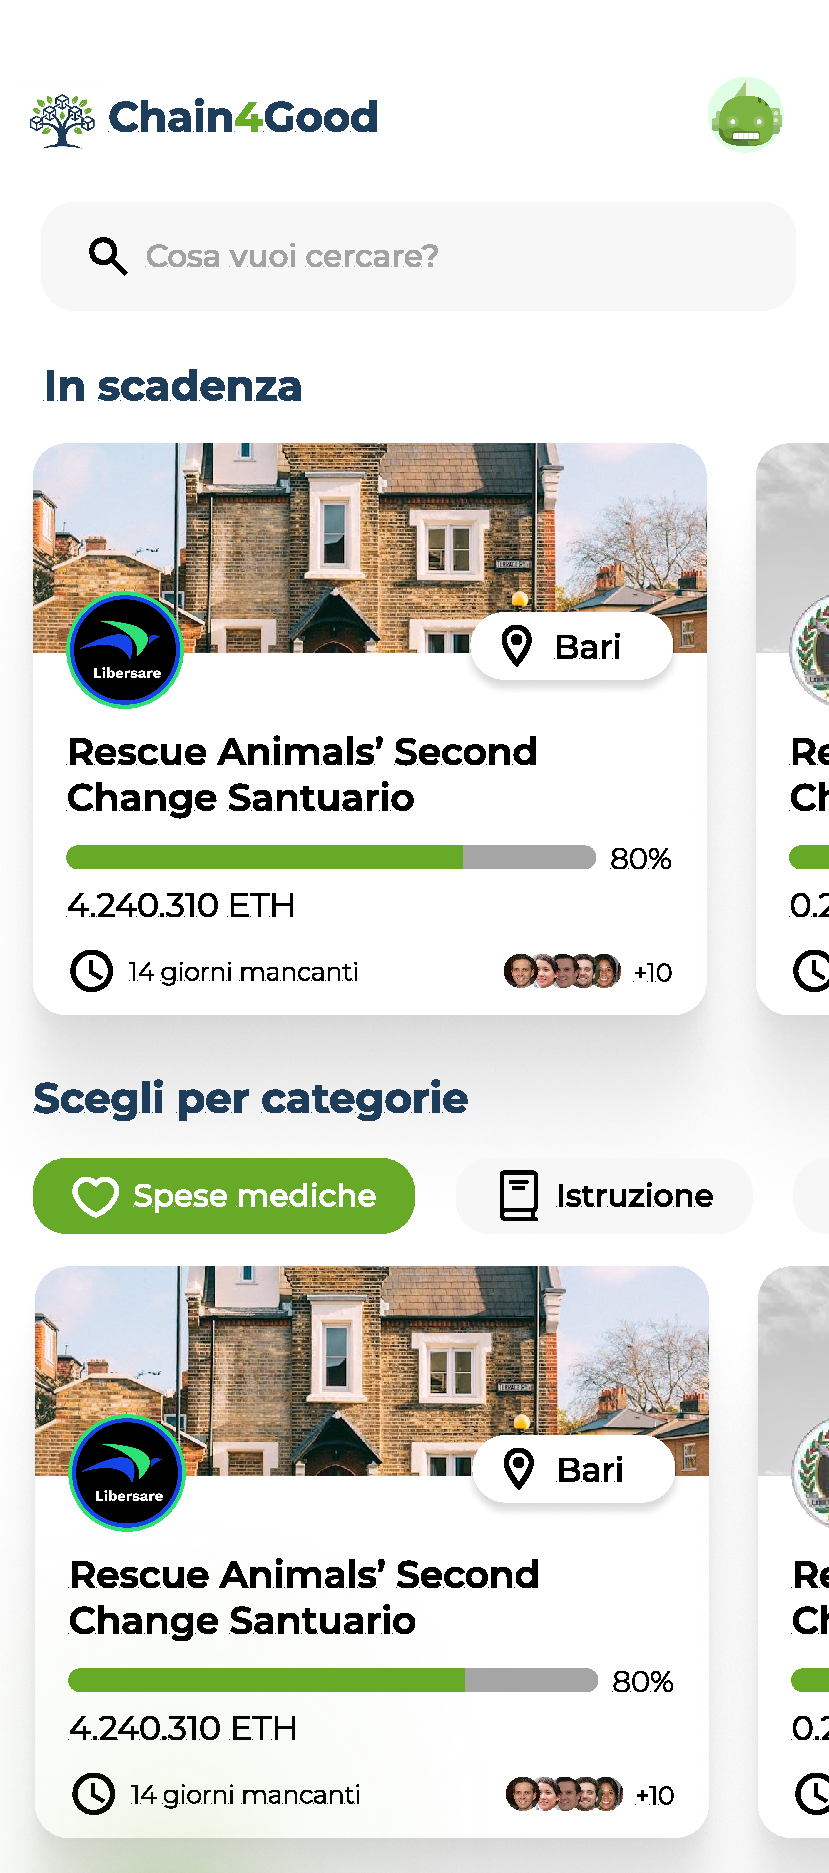
\includegraphics[width=0.37\textwidth]{images/Home_nuova.pdf}
	\caption{Dashboard del donatore}
	\label{fig:dashboard-donatore}
 \end{figure}

\subsection{Creazione progetto}
	La creazione di un progetto costituisce l’atto attraverso il quale il beneficiario formalizza la propria proposta sulla piattaforma. Tale procedura si articola in due step (\ref{fig:inserimento progetto}):

\begin{itemize}
	
	\item Step 1: l'Ente è tenuto a specificare le informazioni fondamentali del progetto, quali il nome, la categoria di appartenenza, l’obiettivo economico e il termine temporale della raccolta fondi. \\ 
	Gli ultimi due parametri permettono di automatizzare la gestione delle risorse in modalità \textit{trustless}, in quanto vengono utilizzati dallo \textit{Smart Contract} per determinare l’esito della campagna di \gls{cf};
	
	\item Step 2: prevede l’inserimento di un piano dettagliato delle spese, oltre ad una descrizione approfondita del progetto e un’immagine di copertina. Tale prospetto non assolve solo finalità informative, ma contribuisce ad incrementare la credibilità dell'iniziativa e a consolidare il rapporto di fiducia con i donatori. 
	
\end{itemize}


\subsection{Inserimento e valutazione spesa}
A differenza dei sistemi centralizzati in cui l'Ente ha piena e immediata disponibilità del \textit{budget} donato, l’architettura proposta prevede che i fondi raccolti rimangano vincolati all'interno di uno \textit{Smart Contract}. \\
Per poter accedere a tali risorse, il beneficiario deve formalizzare una "Richiesta di Spesa" (\ref{fig:valutazione-spesa}) attraverso l'inserimento dei seguenti parametri: nome della spesa, importo richiesto, finalità dell'esborso e preventivo. \\
A seguito della sottomissione, la richiesta viene sottoposta a un meccanismo di valutazione decentralizzato, basato sul voto dei donatori che hanno contribuito al finanziamento del progetto, i quali sono tenuti a esprimere un parere favorevole o contrario.
Coerentemente con la natura della piattaforma, il sistema di voto attribuisce lo stesso peso a ciascun partecipante, indipendentemente dall’importo della donazione effettuata. Questa scelta progettuale è finalizzata a evitare che il potere decisionale risulti influenzato dalla capacità economica dei singoli utenti.\\
Al fine di assicurare un utilizzo progressivo e verificabile delle risorse raccolte, inoltre, la presentazione di una nuova richiesta di spesa è subordinata al caricamento della prova di acquisto relativa all’ultima richiesta precedentemente approvata. 
Tale approccio serve per garantire un utilizzo progressivo e verificabile dei fondi raccolti, e ad assicurare la conformità delle spese per le finalità dichiarate. 

\begin{figure}[t]
	\centering
	\begin{minipage}{0.37\textwidth}
		\centering
		\includegraphics[width=\textwidth]{images/nuovo_progetto1.pdf}
	\end{minipage}
	\hspace{1.5cm}
	\begin{minipage}{0.37\textwidth}
		\centering
		\includegraphics[width=\textwidth]{images/NuovoProgetto 2.pdf}
	\end{minipage}
	\caption{Inserimento di un nuovo progetto}
	\label{fig:inserimento progetto}
\end{figure}


\subsubsection{Meccanismo di validazione}
Per evitare lo stallo decisionale, lo \textit{Smart Contract} è stato programmato per agire secondo le seguenti regole:
\begin{itemize}
	\item la richiesta di spesa è approvata se la maggioranza dei votanti ($\ge 50\%$) esprime un parere favorevole;

	\item In caso di parità tra voti favorevoli e contrari, la richiesta è considerata approvata;
	\item in presenza di una partecipazione parziale, la soglia di maggioranza viene ricalcolata esclusivamente in funzione dei soli voti espressi;
	\item qualora non venga registrata alcuna attività di voto entro il periodo di valutazione (pari a tre giorni), il sistema approva automaticamente la richiesta;
\end{itemize}

Al soddisfacimento dei requisiti di approvazione, lo \textit{Smart Contract} esegue in modo autonomo e irreversibile il trasferimento della somma raccolta verso il \textit{wallet} del beneficiario. 


\begin{figure} [h]
	\centering
	\begin{minipage}{0.37\textwidth}
		\centering
		\includegraphics[width=\textwidth]{images/nuova_spesa.pdf}
	\end{minipage}
	\hspace{1.5cm}
	\begin{minipage}{0.37\textwidth}
		\centering
		\includegraphics[width=\textwidth]{images/valutazione_spesa.pdf}
	\end{minipage}
	\caption{Valutazione di una richiesta di spesa}
	\label{fig:valutazione-spesa}
\end{figure}









